\subsection{Candidate and Monitored Set Sizes}
\label{subsec:setsizes}

We now quantify the scalability gains obtained with our bound on the
candidate set.  We compute the sizes of the general and bounded
candidate sets $\mathcal{C}(v)$ and $\mathcal{B}(v)$ for all path
changes in our poisoning experiments and also the sizes of the general
and bounded monitored sets $M(v)$ and $T(v)$.  We use our exhaustive
poisoning experiments (the same used in \S~5.2) as we need topology
information as complete as possible to compute $\mathcal{C}(v)$ and
$M(v)$.  Using our exhaustive poisonings also increases the variability
of observed path changes (\ie path changes we would rarely observe in
practice).  The further an AS is from the origin AS (\ie our BGP-Mux
providers), the larger its candidate and monitored sets.  We compute
candidate and monitored sets for the ASes where we have vantage points
as they are the furthest from the origin AS in our dataset.  

\begin{figure}
\begin{center}
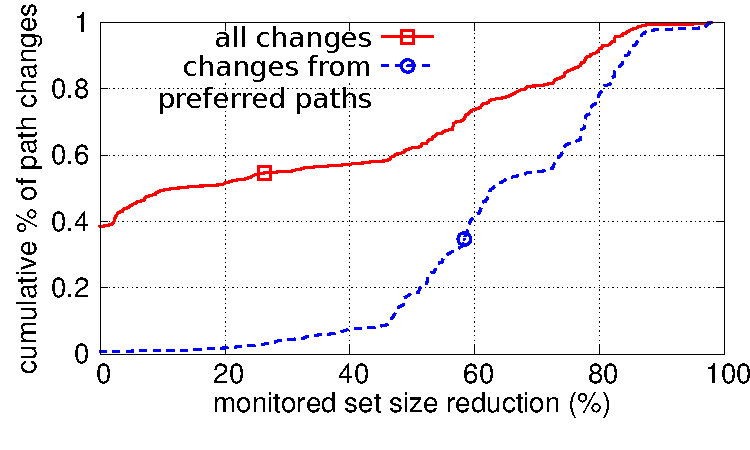
\includegraphics[width=1.0\columnwidth]{figs/scalability_monset_gains.pdf}
\caption{Our bound on the candidate set size allows us to reduce the
number of ASes we have to monitor to perform root cause analysis.}
\label{fig:setsizes}
\end{center}
\end{figure}

\fig~\ref{fig:setsizes} shows the distribution of the reduction in
monitored set size (from general to bounded) across all path changes in
the data set.  Overall, we reduce the monitored set size by more than
50\% for 38\% of path changes.  The bounded candidate set is identical
to the general candidate set for around 40\% of the path changes (where
the solid line intersects the $y$-axis).  This happens whenever an AS is
using its least preferred path (\ie we have to monitor all other paths
that are more preferred).  Even if an AS is not using its least
preferred path, the number of ASes to monitor quickly converges to the
general monitored set as the number of more preferred paths we need to
monitor increases.  The dashed line shows that the monitored set size
reduction is significantly higher when an AS changes from its most
preferred path to a less preferred one.  The reduction in candidate set
sizes is much smaller (not shown), as induced path changes are rare in
practice and we do not observe any 3-level induced path change.
